\chapter{Návrh}\label{chap:design}

V~tejto kapitole predstavíme základný algoritmus a postupne sa budeme venovať jeho jednotlivým častiam. Budeme sa venovať metódam na zlepšenie úspešnosti klasifikátora a porovnáme rôzne prístupy. 
\bigskip

\section{Základný algoritmus}

Základný algoritmus (Obr. \ref{fig:base_alg}) vyzerá nasledovne: 
Najskôr sa získa obraz z webkamery. Ten sa potom spracuje a následne sa rozsegmentuje na jednotlivé pohybujúce sa objekty.
Každý z týchto segmentov sa predloží klasifikátoru, ktorý rozhodne, či daný segment je, alebo nie je ruka. Zo všetkých segmentov je vybratý ten, o ktorom si je klasifikátor najviac istý, že je ruka (a zároveň spĺňa danú hranicu). Z vybratého segmentu sa vypočíta bod, ktorý je braný ako pozícia ruky. Tento bod je pridaný do postupnosti bodov, o ktorých sa ďalej rozhodne, či tvoria niektoré gesto. Ak klasifikátor gesta detekuje nejaké gesto, vykoná sa príslušná akcia - simulácia stlačenia niektorej klávesy - a postupnosť sa vymaže. Ak sa dlhšiu dobu v obraze nevykonala žiadna zmena a klasifikátor gesta nezistil žiadne gesto, postupnosť sa tiež vymaže.

\begin{figure}[htp]
    \centering
%    \includegraphics[scale=1]{img/00/extern-drive-encryption.1.mps}
    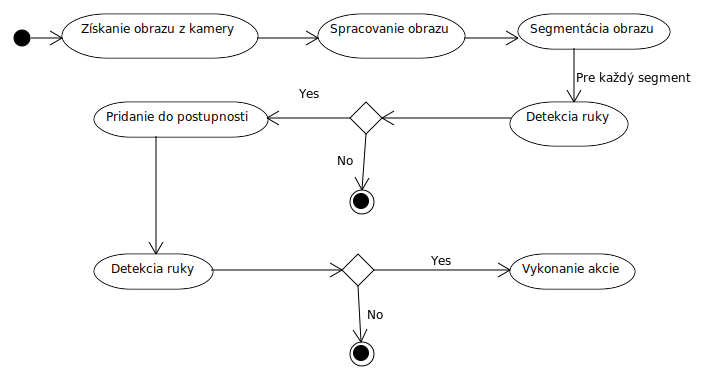
\includegraphics[width=\textwidth]{images/BaseAlgorithm}
%    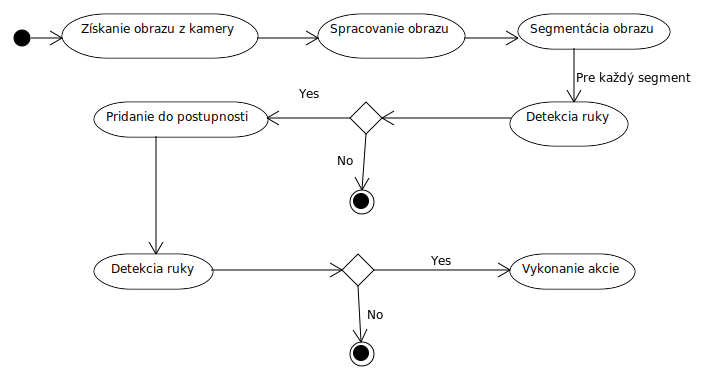
\includegraphics[scale=1]{images/BaseAlgorithm}
    \caption{Základný algoritmus}
    \label{fig:base_alg}
\end{figure}

\subsection{Rozdielový obraz}\label{chap:diffimg}

Základ pre predspracovanie a segmentáciu tvorí takzvaný \textbf{rozdielový obraz}. Rozdielový obraz je obraz, ktorý vznikne odčítaním 2 po sebe idúcich čiernobielych obrázkov v absolútnej hodnote. Tento obraz obsahuje zmeny - pohybujúce sa objekty. Statické objekty sa tam teda nevyskytnú, čo nám umožní ich veľmi ľahko odfiltrovať. V tomto obraze sa vyskytnú obrysy pohybujúcich sa objektov, pretože ku zmenám dochádza najviac na hranách. Podľa rýchlosti pohybu môžu byť obrysy hrubšie, alebo tenšie. 

\subsection{Predspracovanie vstupného obrazu}\label{chap:preprocess}

%Našim cieľom je čo najlepšie zachytiť pohybujúcu sa ruku.

%Dohodneme sa, že najmenšia zmena (žiadna) bude znázornená bielou a najväčšia čiernou. 

\subsubsection{Odfiltrovanie šumu}
Odfiltrovanie šumu zabezpečí hranica -- \textit{treshold}. Všetky pixle svetlejšie ako určitá konštanta, budú vykreslené bielou. Ideálna hranica je taká, ktorá potlačí šum, ale zachová čo najviac z ostatných zmien -- čiže by mala byť najmenšia možná. Pohybujeme sa v odtieňoch šedej, čiže hodnoty $0\dots 255$. Praktické testy ukázali, že vhodnou hodnotou pre hranicu je 7.

\subsubsection{Rozpitie pixlov}

Kvôli segmentácii potrebujeme aby jednotlivé segmenty boli súvislé. Teda aby obrys ruky tvoril jeden celok.
Ľahko sa nám však môže stať, že obrys ruky je niekde prerušený - nedostatočná zmena, prípadne iné dôvody. Predpokladáme ale, že všetky časti jedného segmentu sú dostatočne blízko. Spojiť segmenty nám teda pomôže rozpitie pixlov. 

%TODO spravnu konštantu, spomenut rozlisenie
Z každého pixla spravíme štvorec s veľkosťou $11\times 11$.
Hodnota 11 pre stranu štvorca sa ukázala ako najvhodnejšia. 
Príliš veľké hodnoty spájajú aj časti, ktoré nepatria do toho istého segmentu, príliš malé zase nespoja časti, ktoré sú ďalej od seba.

\subsection{Segmentácia}\label{chap:segment}
Rozpitý obrázok si teraz vieme predstaviť ako graf, pričom hrana je medzi každými 2 susediacimi pixlami (v štyroch smeroch). Segmentácia je vlastne len nájdenie komponentov v tomto grafe. Na to môžeme použiť napríklad prehľadávanie do šírky. 

Potrebujeme ešte nájsť opísaný obdĺžnik. To spravíme tak, že nájdeme najľavejší, najpravejší, najvrchnejší a najspodnejší bod segmentu.

%TODO mozno zmenit urovne kapitol
\subsection{Predspracovanie segmentov}
\label{sect:segmentpreprocessing}

V tejto časti sa budeme zaoberať jednotlivými segmentami, ktoré budeme predkladať neurónovej sieti, aby nám povedala, či je to ruka, alebo nie.

Každý nájdený obdĺžnik sa naškáluje na veľkosť vstupu pre neurónovú sieť - v našom prípade $128\times 128$ - a normalizuje sa. 

\subsubsection{Normalizácia dát} 
Ideálne vstupy pre neurónovú sieť sú z intervalu $\langle 0,1\rangle$. Pixle čiernobielych obrázkov majú hodnoty $\{0\dots 255\}$. Pri obrázkoch zvolíme pre farbu pozadia hodnotu 0 a pre objekt ostatné hodnoty. Z tohto dôvodu chceme, aby rozdiel v normalizovanej hodnote medzi 0 a 1 bol najväčší a postupne klesal. Preto sme za normalizačnú funkciu zvolili:

$$f(x)=\frac{1}{1+x}$$

Pre normalizáciu fourierovej transformácie sme zvolili tú istú funkciu. %TODO dôvod? 

%TODO Popisat preco je to nutne a v com to pomaha

\todo 

\subsubsection{Fourierova transformácia} \label{sect:ft}
Fourierova transformácia zvykne často pomáhať, keď sa použie na predspracovanie dát pri trénovaní obrazových alebo zvukových vzoriek. Preto sme sa aj my rozhodli vyskúšať aký bude mať vplyv na úspešnosť.

Fourierova transformácia bola použitá na segment ako celok, potom bola prevedená do reálnych čísel ako absolútna hodnota z komplexného čísla a následne normalizovaná.

Konvergencia chyby pri trénovaní bola značne rýchlejšia a použitie transformácie umožnilo dosiahnuť menšiu chybu na trénovacej množine. 

\todo

\subsubsection{Použitie pôvodného namiesto rozdielového obrázka}
Nevýhodou rozdielového obrázka je, že zmena spôsobená pohybom sa v ňom vyskytne dvakrát. Raz na mieste, kam sa objekt posunul a raz na mieste odkiaľ sa posunul. Toto sme chceli eliminovať tak, že sa vyberie ruka z pôvodného obrázka podľa farby. Táto ruka tam bude vždy len raz. Bohužiaľ tento prístup mal viac zlých vlastností ako dobrých.

Pri vyberaní obrázka treba mať nastavené správne parametre, podľa ktorých sa rozhoduje čo pridať do výberu a čo nie. Tieto parametre veľmi závisia od osvetlenia. Navyše osvetlenie sa môže meniť pri pohybe ruky, čo veľmi sťažuje nastavenie správnych parametrov. Pred použitím aplikácie by sa aplikácia musela nakalibrovať, čo znižuje komfort jej použitia.

Ďalší problém je správne tipnúť bod, ktorý patrí ruke, aby sa z neho mohla odštartovať selekcia. Pokiaľ by bola v danom obdĺžniku len dlaň, tak nie je až také ťažké sa správne trafiť - je takmer isté, že kúsok pod stredom obrázka bude dlaň. Bohužiaľ často sa stane, že užívateľ pohne nielen rukou, ale aj predlaktím a segmentačný algoritmus zaradí do segmentu aj predlaktie. Potom sa môže stať, že bod ruky netrafíme.

{\color{red}
Rozhodujúcim problémom však bolo to, že úspešnosť siete na dátach, ktoré ani neobsahovali zle vybraté ruky bola aj tak nižšia ako u rozdielového obrázka (tabuľka \ref{tab:neuraldatacmp}). Preto sme sa rozhodli radšej pridať ďalšie dáta do trénovacej množiny pre rozdielové obrázky. Pri vyhodnocovaní tejto časti sme použili menšiu trénovaciu a testovaciu sadu, ktorá obsahovala cca 350 trénovacích a 300 testovacích vzorov. Sada neobsahovala zle vybraté ruky.
}


\section{Návrh architektúr neurónových sietí}\label{chap:neuralnetarch}

V tejto kapitole si popíšeme rôzne architektúry sietí, ktoré sme vyskúšali a porovnáme ich vlastnosti a úspešnosť pri riešení problému rozpoznania ruky a vyberieme vhodnú architektúru, ktorú potom použijeme v našej aplikácii.

\subsection{Cieľ}

Našim cieľom je vytvoriť vhodnú architektúru neurónovej siete, ktorá bude rozhodovať o danom vstupe, či zodpovedá ruke alebo nie. 
Navrhneme niekoľko typov architektúr, ktoré neskôr porovnáme (\ref{chap:experiments}) a vyberieme najvhodnejšiu z nich, ktorú potom použijeme v aplikácií. 

Neurónová sieť má rozdeliť vstupy do 2 tried - tie, ktoré zodpovedajú rukám a ostatné. Na to využijeme vo všetkých architektúrach jeden výstupný neurón.

\subsection{Typ 1: Viac vrstvová dopredná neurónová sieť}

{\color{red}
\textbf{Viac vrstvová dopredná neurónová sieť} (obr. \ref{fig:ffnn}) je neurónová sieť zložená z viacerých vrstiev neurónov, pričom signál sa šíri len zo spodnejšej vrstve na vyššiu. Viac o tomto type siete nájdete v kapitole \ref{chap:ffnn}.
}
%V našej implementácii siete sa ako vstup každého neurónu berie výstup každého neurónu z predošlej vrstvy. Prvá vrstva dostane pôvodný vstup. 

\subsection{Typ 2: Upravená verzia viac vrstvovej doprednej neurónovej siete}

\begin{figure}[h]
  \begin{center}
    \includegraphics[width=0.3\textwidth]{images/dffnn}
  \end{center}
  \caption{Upravená dopredná neurónová sieť}
  \label{fig:dffnn}
\end{figure}

V upravenej verzii sme upravili spodnú vrstvu siete - tú, ktorá dostáva vstup. Vstup je rozdelený na 16 častí a ku každej časti je pridelených niekoľko neurónov. Každý neurón spracúva len vstupy z jeho časti (obr. \ref{fig:dffnn}). 

Jej výhodou je rýchlosť. Náš vstup má rozmer $128\times 128 = 16384$, čo nie je malé číslo. Rozdelíme ho na 16 častí s veľkosťou $32\times 32 = 1024$. Takto namiesto toho aby každý vstupný neurón počítal s 16384 vstupmi počíta len s 1024, čo je $16\times$ rýchlejšie. Skupina neurónov pridelená danej časti sa stará len o príznaky zo svojej časti a nie je ovplyvňovaná ostatnými časťami. 

Nevýhodou je to, že neuróny sú fixne pridelené na jednotlivé vstupy. V pôvodnej sieti si neuróny sami vyberali, ktoré časti vstupu sú pre nich najvýznamnejšie a mohli tak lepšie pokryť vstup.

\subsection{Typ 3: Rekurentná neurónová sieť}

V predchádzajúcich podkapitolách sme sa zaoberali doprednými sieťami (feedforward), v ktorých sa informácia šírila len smerom od vstupov k výstupu. V rekurentných sieťach máme navyše rekurentné spojenia, cez ktoré sa informácia prenáša v čase. Informácia z jednotlivých neurónov môže byť v ďalšom kroku použitá ako vstupná informácia pre neuróny.

Naša architektúra rekurentnej neurónovej siete vychádza z upravenej doprednej neurónovej siete, s tým, že namiesto obyčajného neurónu používame v niektorej vrstve rekurentný neurón (obr. \ref{fig:recurentneuron}). 

\begin{figure}[htbp]
  \begin{center}
    \includegraphics[width=0.15\textwidth]{images/recneuron}
  \end{center}
  \caption{Rekurentný neurón}
  \label{fig:recurentneuron}
\end{figure}

Rekurentný neurón obsahuje navyše spätnú väzbu. Spätná väzba sa tvári ako ďalší vstup a obsahuje posledný updatenutý výstup toho istého neurónu. Po aktivácii neurónu môžeme updatnuť poslednú aktivačnú hodnotu. Ak to neurobíme, hodnota ostane taká, ako bola predtým. Neurón môžeme aj resetnúť, vtedy sa hodnota vynuluje.

Tento typ siete sme navrhli z ohľadom na už existujúce typy sietí a architektúru aplikácie. Umožňuje nám bez väčšieho zásahu použiť túto sieť tak, aby nám v každom kroku vedela povedať, či sa jedná o ruku alebo nie. Oproti predošlým typom sietí má navyše informáciu o tom ako reagovala sieť na predošlých rukách.

Našu jednoduchú rekurentnú neurónovú sieť trénujeme tiež algoritmom \textit{backpropagation} s tým, že sieti predkladáme postupnosti - vždy v tom istom poradí. Pri kladnej odozve updatujeme rekurentný vstup, ináč nie. Po každej postupnosti zresetujeme rekurentný vstup na 0.

%TODO vysvetlit? 

\todo
